\documentclass{ximera}  
\title{Flowcharts}  
\begin{document}  
\begin{abstract}  
We introduce flowcharts as a way to organize a procedure designed to solve a particular problem.
\end{abstract}  
\maketitle

\section{Flowcharts}
An algorithm is a fixed set of instructions that can be followed to solve a problem. Algorithms take in a set of inputs from a predefined set, perform a series of clearly defined operations, and produce an output meant to solve a particular problem. While it may take a while for an algorithm to produce an answer (say, if the size of the input is large), it should always be the case that the solution to the problem is found in a finite amount of time.

There are several ways to specify an algorithm. For now we will represent our algorithms using a special type of diagram known as a flowchart. As we gain more experience we will be able to transition to other methods for expressing algorithms. We begin with flowcharts because they are a relatively intuitive to use and because you probably have some prior experience with them.

Here, for example, are two different flowcharts that describe how you might accomplish a certain common task. 

\begin{center}
	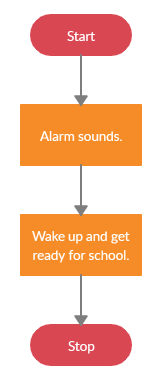
\includegraphics{morning1.png}
\end{center}
\begin{center}
	An example of a morning routine.
\end{center}

\begin{center}
	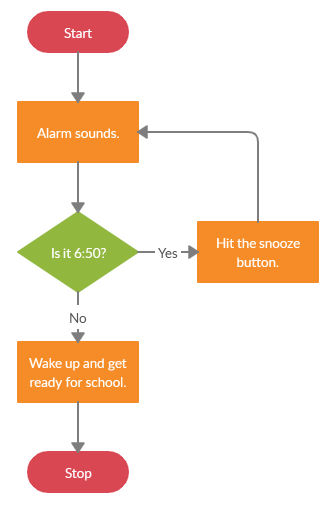
\includegraphics{morning2.png}
\end{center}
\begin{center}
	Another example of a morning routine.
\end{center}

Note that the flowcharts above are not examples of algorithms. The individual steps are too vague to claim that they form a precise set of instructions. The point of these flowcharts is to show how they may help you organize your thoughts in a naturally sequential way.

We use the following conventions for our flowchart compartments (there are others, but these are the main ones we will use). Arrows between the different compartments show how the algorithm progresses from one operation/input/decision to another.

\begin{center}
	
\includegraphics{startstop.png}
\end{center}
\begin{center}
	Beginning or end of the algorithm.
\end{center}

\begin{center}
	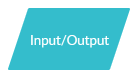
\includegraphics{io.png}
\end{center}
\begin{center}
	Indicates data input or output.
\end{center}

\begin{center}
	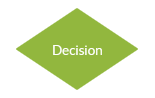
\includegraphics{decision.png}
\end{center}
\begin{center}
	Conditional operation/decision. Typically limited to true/false or yes/no options.
\end{center}

\begin{center}
	
\includegraphics{process.png}
\end{center}
\begin{center}
	A set of operations.
\end{center}

The following flowchart represents a simple algorithm that computes the absolute value of any real number $x$.

\begin{center}
	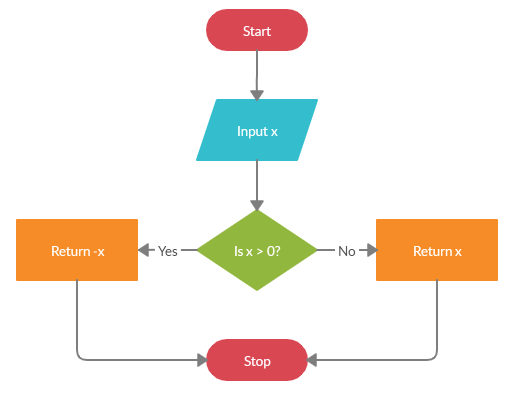
\includegraphics{absalgo.png}
\end{center}
\begin{center}
	An example of an algorithm that computes $|x|$.
\end{center}

\section{Problems}

\begin{question}
	Consider the algorithm given by the flowchart below. Determine the output given each of the following inputs:
	\begin{itemize}
		\item $n = 5 \answer{1}$
		\item $n = -4 \answer{0}$
		\item $n = 2 \answer{0}$
	\end{itemize}
	\begin{center}
	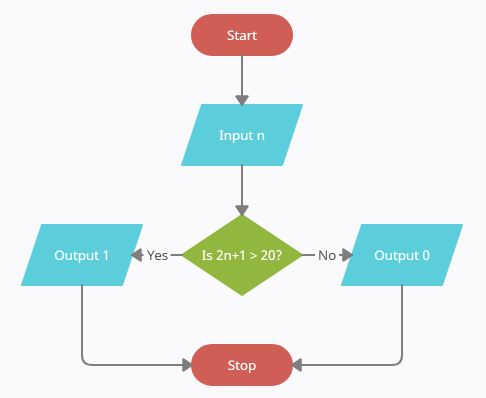
\includegraphics{20bigger.png}
	\end{center}
\end{question}

\begin{question} 
	Develop an algorithm that takes in two inputs $a$ and $b$ and outputs their average. Draw a flowchart for your algorithm.
	\begin{hint}
		Your flowchart should only need 4 compartments: a start compartment, an input compartment, a output compartment giving the average, and a stop compartment. Note that the second hit for this problem is the solution.
	\end{hint}
	\begin{hint}
		\begin{center}
		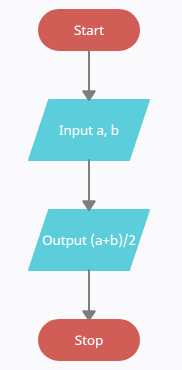
\includegraphics{average.png}
		\end{center}
	\end{hint}
\end{question}
	
\begin{question}
	
\end{question}

\begin{question}
	Consider the following scenario. Suppose that you can buy an avocado at the grocery store for \$1 or 5 avocados for \$3. Develop an algorithm for computing the minimum price for buying at least $n$ avocados where $1\leq n\leq 5$ and draw a flowchart for your algorithm.
	\begin{hint}
		You can modify the algorithm for computing $|x|$. Note that the second hint for this problem is the solution.
	\end{hint}
	\begin{hint}
		\begin{center}
		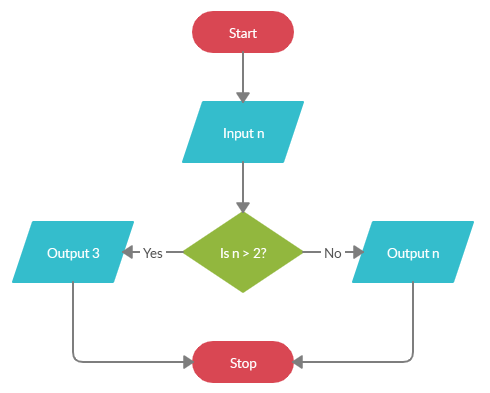
\includegraphics{avocados.png}
		\end{center}
	\end{hint}
\end{question}
\end{document}
